\subsection{Fragen und Antworten zum Text von \textcite{nguyen_multicultural_2010}}
\subsubsection{Wie definieren die Autorinnen Multikulturalismus und multikulturelle Identit"at?}
\begin{itemize}
        \item \textbf{Multikulturalismus} bezeichnet die Ber"uhrung mit und die Internalisierung von zwei oder mehr Kulturen.
        \item \textbf{Multikulturelle Identit"at} bezeichnet das Vorhandensein einer starken Bindung mit diesen Kulturen.
\end{itemize}

\subsubsection{Worauf bezieht sich der Begriff Bikulturalismus? Was ist mit Bilingualismus gemeint?}
Bikulturalismis ist der Spezialfall von Multikulturalismus mit genau zwei Identit"aten. Bilingual sind solche Personen, die zwei Sprachen flie"send sprechen.

\subsubsection{Welche Ziele werden mit multikulturellen Ideologien angestrebt und wieso?}
Multikulturelle Ideologien bef"urworten die Inklusion und Gleichwertigkeit aller vorhandenen Kulturen einer Gesellschaft. Es wird angenommen, dass die Anerkennung der eigenen Kultur und M"oglichkeiten der multikulturellen Interaktion zentral f"ur die eigene Kultur und das Wohlbefinden sind. 

\subsubsection{Wie unterscheiden sich Mitglieder einer ethnischen Minorit"at von Mitgliedern der Majorit"at in Bezug auf multikulturelle Ideologien?}
\begin{itemize}
        \item Mitglieder der Minorit"at bef"urworten Multikulturalismus eher als Mitglieder der Majorit"at. 
        \item positiver Zusammenhang von Multikulturalismus und Selbstvertrauen bei Minorit"atsmitgliedern
        \item positiver Zusammenhang von ethnischer Identifikation und Multikulturalismus bei Minorit"atsmitgliedern
        \item negativer Zusammenhang von ethnischer Identifikation und Multikulturalismus bei Majorit"atsmitgliedern
\end{itemize}

\subsubsection{Nennen sie Beispiele daf"ur, wie sich die Adaption einer multikulturellen Ideologie politisch und gesellschaftlich manifestieren kann!}
\begin{itemize}
        \item doppelte Staatsb"urgerschaft
        \item politische Unterst"utzung von Medien in anderen Sprachen
        \item Feiertage 
        \item Gemeindezentren
        \item Akzeptanz von traditioneller Kleidung und Verhaltensweisen
\end{itemize}



\subsubsection{Worin unterscheiden sich klassische und moderne Akkulturationstheorien? Welche Positionen werden empirisch gest"utzt?}
Klassische Akkulturationstheorien gehen von einem eindimensionalen Konstrukt aus, w"ahrend moderne Ans"atze zwei Dimensionen annehmen. Empirische Befunde st"utzen die moderne Sichtweise.

\subsubsection{Skizzieren sie das Akkulturationsmodell von Berry (2003)!}
Siehe Fig. \ref{fig:nguyen1}
\begin{figure}[hb!]
        \begin{center}
                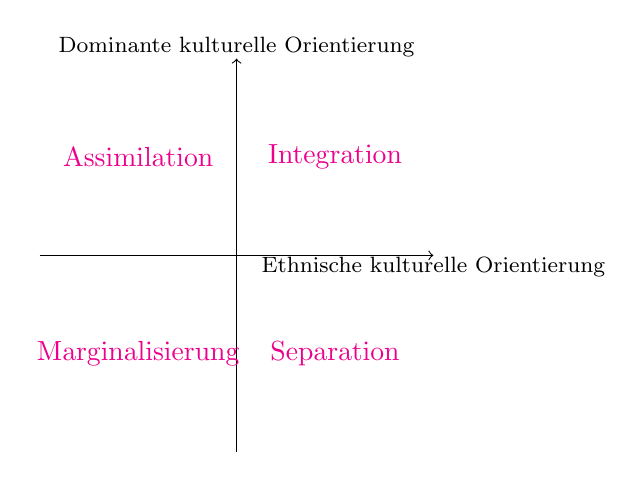
\begin{tikzpicture}
                        [ind/.style={color=magenta},
                        soc/.style={color=cyan},
                        scale=.5]
                        %Koordinatensystem
                        \draw [->] (-5,0) -- (5,0);
                        \draw [->] (0,-5) -- (0,5);
                        \node [font=\footnotesize] at (5,-0.3) {Ethnische kulturelle Orientierung};
                        \node [font=\footnotesize] at (0,5.3) {Dominante kulturelle Orientierung};
                        %Orientierungen
                        \node [ind] (Int) at (+2.5,+2.5) {Integration};
                        \node [ind] (Mar) at (-2.5,-2.5) {Marginalisierung};
                        \node [ind] (Ass) at (-2.5,+2.5) {Assimilation};
                        \node [ind] (Sep) at (+2.5,-2.5) {Separation};
                \end{tikzpicture}
                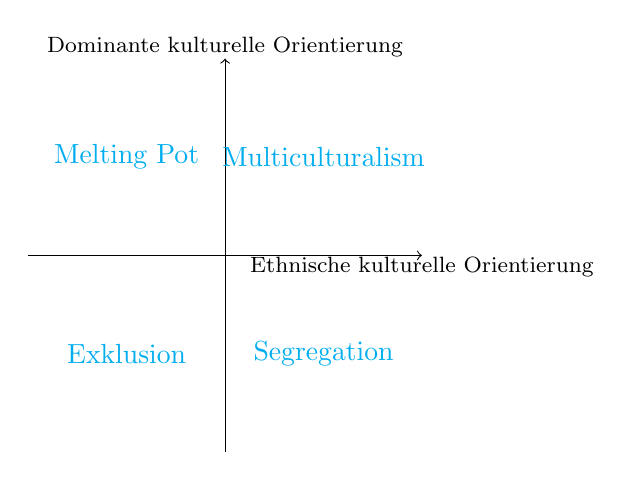
\begin{tikzpicture}
                        [ind/.style={color=magenta},
                        soc/.style={color=cyan},
                        scale=.5]
                        %Koordinatensystem
                        \draw [->] (-5,0) -- (5,0);
                        \draw [->] (0,-5) -- (0,5);
                        \node [font=\footnotesize] at (5,-0.3) {Ethnische kulturelle Orientierung};
                        \node [font=\footnotesize] at (0,5.3) {Dominante kulturelle Orientierung};
                        %Orientierungen
                        \node [soc] at (+2.5,+2.5) {Multiculturalism};
                        \node [soc] at (-2.5,+2.5) {Melting Pot};
                        \node [soc] at (+2.5,-2.5) {Segregation};
                        \node [soc] at (-2.5,-2.5) {Exklusion};
                \end{tikzpicture}
        \end{center}
        \caption{Akkulturationsmodell nach Berry (2003). Links sind die Akkulturationsstrategien auf \textcolor{magenta}{individueller Ebene}, rechts die auch \textcolor{cyan}{gesellschaftlicher Ebene}. Die Achsen gehen (anders als im Studienbrief) von niedrig (links, bzw. unten) nach hoch (rechts, bzw. oben).}
        \label{fig:nguyen1}
\end{figure}

\subsubsection{Was ist mit \emph{cultural frame switching} gemeint?}
Das hin- und herwechseln zwischen kulturellen Orientierungen in Abh"angigkeit der Situation.

\subsubsection{Die Autorinnen schreiben: ``it is important to point out that the acculturation perspective does not presuppose that multicultural individuals internalize and use their different cultures globally and uniformly ''(p. 92). Was ist damit gemeint?}
Verschiedene kulturelle Identit"aten m"ussen nicht in jedem Lebensbereich gleicherma"sen pr"asent sein. Z.B. k"onnte ein Mexikaner in den USA haupts"achlich spanisch sprechen, sich aber trotzdem amerikanischen Werten sehr stark verbunden f"uhlen.

\subsubsection{In welche Typen/Klassen unterteilen (a) LaFromboise et al. (1993), (b) Birman (1994) und (c) Phinney und Devic-Navarro (1997) bikulturelle Personen? Welche Einschr"ankungen/Probleme gehen mit solchen Herausforderungen einher?}
LaFromboise et al. (1993) unterteilen in 2 Klassen: \emph{alternation} und \emph{fusion}.
\begin{itemize}
        \item \textbf{Alternation:} Verhalten passt sich der Situation an (cultural-frame switchers)
        \item \textbf{Fusion:} Orientierung in Richtung einer neuen Kultur
\end{itemize}

\noindent Birman (1994) unterscheidet vier Typen von Individuen:
\begin{itemize}
        \item \textbf{blended:} so wie \emph{fused}
        \item \textbf{instrumental:} Verhalten richtet sich nach beiden Kulturen, Identit"at an keiner von beiden
        \item \textbf{integrated:} Verhalten richtet sich nach beiden, Identit"at nur ethnische Kultur
        \item \textbf{explorers:} Verhalten orientiert sich an dominanter, Identit"at nur an ethnischer Kultur
\end{itemize}

\noindent Phinney und Devich-Navarro (1997) wollen beide Ans"atze integrieren. Sie nehmen zwei Klassen an, die stark an LaFromboise et al. (1993) angelehnt sind:
\begin{itemize}
        \item \textbf{blended biculturals:} Identit"at orientiert sich an beiden Kulturen, kein wahrgenommener Konflikt
        \item \textbf{alternating biculturals:} Identit"at orientiert sich an beiden Kulturen, aber wahrgenommener Konflikt
\end{itemize}

Ein Problem dieser Ans"atze ist  die Vermischung von Verhaltensorientierten und Identit"atorientierten Aspekten. Phinney und Devich-Navarros (1997) Ansatz zielt auf die Identit"at ab, w"ahrend Birmans (1994) Ansatz auf das Verhalten abzielt. LaFromboise et al. (1993( vermischen beides. 

\subsubsection{Wie sollten (bzw. sollten nicht) Akkulturationseinstellungen, Multikulturalismus und Bikulturalismus operationalisert werden? Bergr"unden Sie Ihre Antwort}

Was man machen sollte:
\begin{itemize}
        \item \emph{zweidimensionale Operationalisierung} der kulturellen Orientierungen
        \item \emph{Typologie} mittels Clusteranalyse oder Latent Trait Analyse
        \item \emph{direkte Messung} der Akkulturationsstrategien (mit Einschr"ankungen wg. psychometrischer Probleme)
\end{itemize}

\noindent Was man nicht machen solte:
\begin{itemize}
        \item \emph{eindimensionale Messung.} Hier wird Identifizierung mit einer Kultur gleichgesetzt mit der Nicht-Identifizierung der anderen Kultur.
        \item \emph{Addieren, Subtrahieren oder Multiplizieren} von verschiedenen Orientierungsskalen. Von Vpn mit mittleren Werten wei"s man dann nicht, ob sie auf allen Skalen mittlere Werte angegeben haben, oder auf einer Skala einen hohen  und auf einer anderen einen niedrigen Wert.
        \item \emph{Demographische Variablen zur Akkulturationsmessung.} Akkulturation kann in unterschiedlichen Bereichen in unterschiedlichem Ma"s auftreten. Demographische Variablen eignen sich nicht daf"ur, dass zu erfassen 
\end{itemize}

\subsubsection{Worauf bezieht sich \emph{Bicultural Identity Integration} (BII)? Mit welchen psychologischen Korrelaten h"angt BII zusammen? Aus welchen Komponenten setzt sich BII zusammen?}
BII bezieht sich auf das Ausma"s, in dem Personen ihre beiden kulturellen Identit"aten als gut vereinbar oder als in Konflikt stehend betrachten. Egal, ob hohe oder niegrige Werte f"ur BII erreicht werden, die Identit"at orientiert sich an beiden Kulturen. Vgl. dazu auch Abbildung \ref{fig:bii}.

\begin{figure}[<+htpb+>]
        \begin{center}
                \begin{tikzpicture}
                        [predict/.style={ellipse, draw, text centered, text width=3cm, node distance=3cm},
                        main/.style={ellipse, draw, text centered, thick},
                        correl/.style={ellipse, draw, text centered, text width=3cm,},
                        manifest/.style={rectangle, draw, text centered, rounded corners, font=\footnotesize, node distance=0.2cm}]
                        %Praediktoren und BII
                        \node [main](bii) at (+9,+0) {BII};
                        \node [predict] (dis) [above left=of bii] {Kulturelle Distanz {\footnotesize Kompartmentalisierung vs. "Uberlappung}};
                        \node [predict] (con) [below left= of bii]{Kultureller Konflikt {\footnotesize Spannung vs. Harmonie}};
                        \draw [->] (dis) -- (bii);
                        \draw [->] (con) -- (bii);
                        %Korrelate
                        \node [correl][above left=1cm of dis] (korr11) {Probleme in sozialen Interaktionen};
                        \node [correl][below left=1cm of dis] (korr12) {kontextuelle Herausforderungen};
                        \node [correl][above left=of con] (korr21) {Intrapersonelle Belastungen};
                        \node [correl][below left=of con] (korr22) {Interpersonelle Belastungen};
                        \draw [->] (korr11) -- (dis);
                        \draw [->] (korr12) -- (dis);
                        \draw [->] (korr21) -- (con);
                        \draw [->] (korr22) -- (con);
                        %Manifestationen der Korrelate
                        \node [manifest, above left=of korr11] {Wahrnehmung des eigenen Akzents};
                        \node [manifest, left=of korr11] {Close Mindedness};
                        \node [manifest, left=of korr12] (man1) {kulturell nicht diverse Lebensumgebung};
                        \node [manifest, above =of man1] {sprachliche Schwierigkeiten};
                        \node [manifest, above left=of korr21] {Neurotische Disposition};
                        \node [manifest, below left=of korr21] {wahrgenommene Diskriminierung};
                        \node [manifest, left=of korr22] {Belastungen in interkulturellen Beziehungen};
                \end{tikzpicture}
        \end{center}
        \caption{Zusammenh"ange und Wirkungswege von BII. Kultureller Konflikt und Kulturelle Distanz f"uhren zu BII, es handelt sich also um ein formatives Modell. Praediktoren von Kulturellen Konflikt und Kultureller Distanz sind ebenfalls zu sehen.}
        \label{fig:bii}
\end{figure}

\subsubsection{Welche pers"onlichkeits-, leistungs-, und kontextbezogene Antezedenzien h"angen mit cultural distance und cultural conflict zusammen?}
Vgl. dazu Abbildung \ref{fig:bii}.

\subsubsection{Anhand welcher Kriterien können multikulturelle Personen in f"unf Gruppen eingeteilt werden? Um welche f"unf Gruppen handelt es sich? Wie h"angt BII mit diesen Kriterien und den f"unf Gruppen zusammen?}
Basierend auf \emph{Freiwillligkeit, Mobilit"at} und \emph{Dauer} k"onnen die folgenden f"unf Gruppen unterschieden werden:
\begin{itemize}
        \item Immigranten
        \item Fl"uchtlinge
        \item Sojourners
        \item Ethnische Minorit"aten
        \item Eingeborene
\end{itemize}

Zum Zusammenhang mit BII: Immigranten und Sojourners kommen freiwillig und k"onnen auch wieder gehen. Sie sollten sich also eher auf M"oglichkeiten im Gastland fokussieren, weniger auf Konflikte. Bei Fl"uchtlingen und Eingeborenen ist der Kontakt mit der dominanten Kultur oft erzwungen. Konflikte sollten hier zum Tragen kommen. Bei ethnischen Minorit"aten ist es schwieriger zu sagen. Die erste Generation k"onnte eher den Konflikt zwischen den Kulturen wahrnehmen, w"ahrend nachfolgende Generationen eher keinen Konflikt sehen.

\subsubsection{Welche Effekte kann Multikulturalismus für Individuen und Gesellschaften haben? Welche Variablen moderieren diese Effekte? Welche Ansatzpunkte f"ur die community-psychologische Praxis ergeben sich daraus?}
Auf individueller Ebene kann Multikulturalismus zu besserer \emph{psychologischer und soziokultureller Anpassung} f"uhren. Es besteht au"serdem ein Zusammenhang mit \emph{akademischem Erfolg}, der wiederum der ganzen Gesellschaft dient. Moderiert wird der Zusammenhang von eher kontextuellen Variablen. Wer niemals akzeptiert wird, kann auch schlecht eine integrierte Identit"at entwickeln. Auf der anderen Seite geht das auch nciht, wenn man nie mit ethnischen Minderheiten in Kontakt kommt.





